\chapter{माइक्रोबायोम और सहजीविताएँ}\label{ch:b3:microbiomes}

आप कोई अड़तीस लाख करोड़ जीवाणु ढोते हैं, यानी अपनी हर कोशिका पर लगभग
एक, और उनमें से अधिकांश आपकी आँत के अंतिम मीटर में, जहाँ उनका भार आपके
मस्तिष्क जितना है और जहाँ वे आपसे सौ गुना अधिक जीन ढोते हैं। इनमें से
एक भी बिना पाला गया कोई चूहा अपना भार बनाए रखने के लिए तिहाई अधिक भोजन
माँगता है, उसकी प्रतिरक्षा-प्रणाली अविकसित रह जाती है, और उसका व्यवहार
अजीब होता है। कोई मटर का पौधा अपनी शर्करा का दसवाँ भाग अपनी जड़ों की
ग्रंथिकाओं में बसे जीवाणुओं को खिलाता है और बदले में अपनी नाइट्रोजन
पाता है; सारे थलीय पौधों के चार-पाँचवें भाग अपनी जड़ों को लपेटे कवकों के
साथ शर्करा के बदले फ़ॉस्फ़ेट का व्यापार करते हैं, जैसा वे चालीस करोड़
वर्षों से कर रहे हैं; और कोई प्रवाल ऐसा प्राणी है जो अपनी कोशिकाओं के
भीतर शैवाल की खेती करता है और तब मर जाता है जब समुद्र इतना गरम हो जाए
कि वह उन्हें निकाल बाहर करे। सजीव व्यष्टि नहीं, संघ हैं, और यह अध्याय
इन साझेदारियों का जीव-विज्ञान बताता है: उनकी गिनती और लक्षण-वर्णन
अनुक्रमण से कैसे होते हैं, साझेदार क्या-क्या बदलते हैं, इस विनिमय पर
मोल-भाव और चौकसी कैसे होती है, और कुछ साझेदार अंततः कोशिकांग क्यों बन
जाते हैं।

\section{साथ रहने के शब्द}

\begin{definition}[सहजीविता]\label{def:b3:microbiomes:symbiosis}
\index{सहजीविता}\index{सहोपकारिता}\index{सहभोजिता}\index{होलोबायोन्ट}\index{माइक्रोबायोम}\index{ऊर्ध्वाधर संचरण}
\emph{सहजीविता} भिन्न जातियों के जीवों का टिकाऊ, घनिष्ठ साहचर्य है; वह
\emph{सहोपकारिता} है यदि दोनों को लाभ हो, \emph{सहभोजिता} यदि एक को लाभ
हो और दूसरे पर कोई असर न पड़े, और परजीविता यदि एक को दूसरे की कीमत पर
लाभ हो --- और वही जोड़ी परिस्थितियों के साथ इस रेखा पर सरक सकती है।
कोई \emph{अंतःसहजीवी} अपने परपोषी की कोशिकाओं के भीतर रहता है; कोई
\emph{अनिवार्य} साथी अकेला जी नहीं सकता। सहजीवी \emph{ऊर्ध्वाधर} रूप
से संचरित होते हैं, माता-पिता से संतति तक (माहू के \emph{Buchnera}
अंडे से होकर जाते हैं), या \emph{क्षैतिज} रूप से, हर पीढ़ी में नए सिरे
से पर्यावरण या दूसरे परपोषियों से पाए जाते हैं (स्क्विड के
\emph{Vibrio}, मानव आँत के जीवाणु)। \emph{माइक्रोबायोम} किसी आवास ---
कोई आँत, कोई पत्ती का पृष्ठ, मिट्टी का एक ग्राम --- के सूक्ष्मजीवों का
पूरा समुदाय है, और \emph{होलोबायोन्ट} कोई परपोषी अपने माइक्रोबायोम के
साथ है, जिसे उस इकाई की तरह देखा जाता है जो प्राकृतिक वरण को दिखती है।
\end{definition}

\begin{example}[तीन अनिवार्य साथी]\label{ex:b3:microbiomes:obligate}
माहू का \emph{Buchnera} बीस करोड़ वर्षों से अपने परपोषी की कोशिकाओं के
भीतर रहता है, वे अनिवार्य ऐमीनो अम्ल बनाता है जो फ़्लोएम-रस में नहीं
होते, और उसने अपना जीनोम सिकोड़कर \qty{640}{kb} कर लिया है --- अपने
स्वतंत्र-जीवी नातेदारों का सातवाँ भाग --- क्योंकि वह हर वह जीन खो
बैठा जिसे अब परपोषी जुटाता है। जीवाणु \emph{Wolbachia}, जो कीट जातियों
के दो-तिहाई में मिलता है, केवल अंडों से संचरित होता है, और इसीलिए उसने
मादाओं के पक्ष में विकास किया है: वह नर भ्रूण मार देता है, उन्हें मादा
बना देता है, या असंक्रमित मादाओं के अंडे संक्रमित नरों से निषेचित होने
पर मरवा देता है (\emph{कोशिकाद्रव्यी असंगति}), जिससे वह किसी समष्टि में
फैल जाता है; उसे ढोते मच्छर डेंगू खराब ढंग से संचरित करते हैं, और
उन्हें छोड़ने से कई शहरों में डेंगू घटा है। अमीबा \emph{Paulinella} ने
लगभग दस करोड़ वर्ष पहले कोई सायनोजीवाणु भीतर लिया था जो अब न ठीक-ठीक
जीवाणु है, न ठीक-ठीक हरितलवक --- प्रकाश-संश्लेषी कोशिकांगों का कोई
दूसरा, स्वतंत्र उद्गम, बीच रास्ते में पकड़ा गया।
\end{example}

\section{किसी समुदाय की गिनती}

\begin{method}[अनुक्रमण से किसी माइक्रोबायोम का लक्षण-चित्र]\label{met:b3:microbiomes:16s}
\index{16S rRNA अनुक्रमण}\index{मेटाजीनोमिकी}\index{प्रचालनात्मक वर्गिकी इकाई}
अधिकांश सूक्ष्मजीव संवर्धित नहीं किए जा सकते; उनकी गिनती उनके DNA से
होती है। (1) प्रतिदर्श से DNA निकालिए --- मल, मिट्टी, किसी झिल्ली पर
छाना गया समुद्री जल। (2) या तो लघु-उपइकाई राइबोसोमी RNA के जीन
(\emph{16S}) को उसके सार्वत्रिक क्षेत्रों से मेल खाते प्राइमरों से
प्रवर्धित कीजिए और उनके बीच के परिवर्ती क्षेत्र अनुक्रमित कीजिए ---
कोई \emph{ऐम्प्लिकॉन} सर्वेक्षण, सस्ता, जो जीवाणुओं को लगभग वंश तक
पहचानता है और उन्हें \omterm{def:b3:genomics:ngs}{वाचनों} की संख्या से गिनता है; या सारा DNA
अनुक्रमित कीजिए --- \emph{शॉटगन मेटाजीनोमिकी}, जो जीन और पूरे जीनोम
बरामद करती है और इसलिए बताती है कि वह समुदाय क्या कर सकता है, न कि
केवल वहाँ कौन है। (3) \omterm{def:b3:genomics:ngs}{वाचनों} को अनुक्रम-प्रभेदों में या
\emph{\omterm{met:b3:microbiomes:16s}{प्रचालनात्मक वर्गिकी इकाइयों}} में गुच्छित कीजिए (OTU, किसी
``जाति'' के लिए परंपरा से \qty{97}{\%} समरूपता पर), उन्हें आँकड़ाकोशों
से तुलना करके अभिहित कीजिए (\cref{ch:b3:bioinformatics}), और प्रति
प्रतिदर्श गिनतियाँ सारणीबद्ध कीजिए। (4) किसी प्रतिदर्श के भीतर विविधता
निकालिए और प्रतिदर्शों के बीच संघटन की तुलना कीजिए। ये गिनतियाँ सापेक्ष
हैं --- किसी प्रतिदर्श के \omterm{def:b3:genomics:ngs}{वाचन} किसी नियत योग तक जुड़ते हैं --- और
निष्कर्षण, प्राइमरों तथा प्रतिलिपि-संख्या से पक्षपाती होती हैं, इसलिए
एक ही ढंग से संसाधित प्रतिदर्शों के बीच के अंतर वहाँ भरोसेमंद हैं जहाँ
निरपेक्ष संख्याएँ नहीं।
\end{method}

\begin{definition}[विविधता]\label{def:b3:microbiomes:diversity}
\index{जाति समृद्धि}\index{शैनन सूचकांक}\index{सिम्पसन सूचकांक}\index{विरलन}
$S$ जातियों वाले किसी समुदाय के लिए, जिसकी सापेक्ष प्रचुरताएँ $p_{1},\dots,
p_{S}$ हों ($\sum p_{i} = 1$): \emph{समृद्धि} $S$ है;
\emph{शैनन सूचकांक} $H = -\sum_{i} p_{i}\ln p_{i}$ यादृच्छिक रूप से
खींचे गए किसी व्यष्टि की जाति के बारे में अनिश्चितता नापता है, और
$e^{H}$ उतनी ही प्रचुर जातियों की वह संख्या है जो वही अनिश्चितता देती
(जातियों की प्रभावी संख्या); \emph{सिम्पसन सूचकांक}
$D = \sum_{i} p_{i}^{2}$ यह प्रायिकता है कि यादृच्छिक रूप से खींचे गए
दो व्यष्टि एक ही जाति के हों, और $1/D$ कोई दूसरी प्रभावी संख्या है, जो
आम जातियों की ओर भारित है। समृद्धि इस पर निर्भर करती है कि कितने
व्यष्टि देखे गए हैं: कोई \emph{विरलन वक्र} मिली जातियों को प्रतिदर्शित
व्यष्टियों की संख्या के सामने आलेखित करता है, और तब चपटा हो जाता है जब
अधिकांश जातियाँ देखी जा चुकी हों।
\end{definition}

\begin{theorem}[विरलन]\label{thm:b3:microbiomes:rarefaction}
\index{विरलन!सूत्र}\index{गुड का आच्छादन}
किसी प्रतिदर्श में $N$ व्यष्टि हैं और $S$ जातियाँ, जिनमें $N_{i}$
व्यष्टि जाति $i$ के हैं। बिना प्रतिस्थापन के खींचे गए $n$ व्यष्टियों के
किसी यादृच्छिक उप-प्रतिदर्श में जातियों की प्रत्याशित संख्या है
\[
E[S_{n}] = \sum_{i=1}^{S}\left[1 - \frac{\binom{N - N_{i}}{n}}
{\binom{N}{n}}\right],
\]
जो $n$ के साथ चढ़ती है और $S$ के बराबर हो जाती है जब $n = N$। भिन्न
आकारों के दो प्रतिदर्शों की तुलना दोनों को एक ही $n$ तक विरल करके की
जाती है। समुदाय के उन व्यष्टियों का अंश जो अब तक न देखी गई जातियों के
हैं, \emph{गुड के आच्छादन} से आँका जाता है: लगभग $f_{1}/N$, जहाँ
$f_{1}$ ठीक एक बार देखी गई जातियों (एकाकियों) की संख्या है।
\end{theorem}
\begin{proof}
जाति $i$ उप-प्रतिदर्श से ठीक तब अनुपस्थित है जब सारे $n$ व्यष्टि शेष
$N - N_{i}$ में से खींचे जाएँ, जो $\binom{N - N_{i}}{n}$ ऐसे
उप-प्रतिदर्शों में होता है, समान रूप से संभाव्य कुल $\binom{N}{n}$ में
से; इसलिए जाति $i$ प्रायिकता $1 - \binom{N-N_{i}}{n}/
\binom{N}{n}$ से उपस्थित होती है, और उपस्थित जातियों की प्रत्याशित
गिनती इन प्रायिकताओं का योग है (संकेतकों के योग की प्रत्याशा)। हर पद
$n$ के साथ बढ़ता है, और $n = N$ पर अंश का हर द्विपद शून्य है। गुड का
आकलन: अगला खींचा गया व्यष्टि किसी अनदेखी जाति का लगभग उसी प्रायिकता से
होता है जिससे प्रतिदर्श का कोई यादृच्छिक रूप से चुना व्यष्टि अपनी तरह
का अकेला था, $f_{1}/N$ (गुड, 1953); उसका औचित्य यहाँ स्वीकार कर लिया
गया है।
\end{proof}

\begin{example}[दो आँतें]\label{ex:b3:microbiomes:two-guts}
किसी एक व्यक्ति के $1000$ \omterm{def:b3:genomics:ngs}{वाचनों} के प्रतिदर्श से $150$ जातियाँ निकलती
हैं, जिनका $H = 3.5$ है और जिनमें $40$ एकाकी हैं; किसी दूसरे के
$5000$ \omterm{def:b3:genomics:ngs}{वाचनों} के प्रतिदर्श से $260$ जातियाँ। दूसरा ज़रूरी नहीं कि अधिक
विविध हो: उसका प्रतिदर्शन पाँच गुना गहरा था, और उसे $1000$ \omterm{def:b3:genomics:ngs}{वाचनों} तक
विरल करने पर $150$ ही मिल सकती हैं। पहले प्रतिदर्श का आच्छादन $1 - 40/1000 =
\qty{96}{\%}$ है: उस आँत के चार प्रतिशत जीवाणु उन जातियों के हैं जो उस
प्रतिदर्श ने कभी नहीं देखीं, और कोई गहरा प्रतिदर्श उन्हें पा लेगा।
प्रभावी संख्याएँ --- $e^{3.5} \approx 33$ जातियों जितनी समरूपता,
$150$ की समृद्धि के सामने --- कहती हैं कि कुछ ही जातियाँ हावी हैं, और
हर आँत ऐसी ही दिखती है।
\end{example}

\begin{omfigure}
\begin{tikzpicture}
\begin{axis}[
  width=0.68\linewidth, height=5.6cm,
  axis x line=bottom, axis y line=left,
  xmin=0, xmax=5000, ymin=0, ymax=300,
  xlabel={प्रतिदर्शित वाचन, $n$}, ylabel={देखी गई जातियाँ},
  xlabel style={font=\small, at={(axis description cs:0.5,-0.12)}, anchor=north}, ylabel style={font=\small},
  tick label style={font=\small}, xtick={0,1000,2000,3000,4000,5000}, ytick={0,100,150,200,260},
  clip=false,
]
\addplot[very thick, omDef, domain=0:5000, samples=60] {260*(1-exp(-x/1500))};
\addplot[very thick, omThm, domain=0:1000, samples=30] {150*(1-exp(-x/300))*1.0};
\addplot[very thick, omThm, dashed, domain=1000:5000, samples=30] {150*(1-exp(-x/300))*1.0 + 8*(1-exp(-(x-1000)/2000))};
\draw[dashed, gray] (axis cs:1000,0) -- (axis cs:1000,300);
\node[font=\scriptsize, omDef, anchor=north west] at (axis cs:1200,292) {दूसरी आँत: $260$ जातियाँ, $5000$ वाचनों पर};
\node[font=\scriptsize, omThm, anchor=north east] at (axis cs:4900,140) {पहली आँत: $150$ जातियाँ, $1000$ पर, अपने पठार के पास};
\node[font=\scriptsize, gray, anchor=south west] at (axis cs:1050,10) {तुलना के लिए यहाँ विरल कीजिए};
\end{axis}
\end{tikzpicture}

{\small \omterm{def:b3:microbiomes:diversity}{विरलन} वक्र। मिली जातियाँ प्रतिदर्शित \omterm{def:b3:genomics:ngs}{वाचनों} के साथ चढ़ती हैं और
तब चपटी हो जाती हैं जब समुदाय चुक जाए; दो प्रतिदर्शों की तुलना एक ही
गहराई पर होती है। यहाँ दूसरी आँत $5000$ \omterm{def:b3:genomics:ngs}{वाचनों} पर भी चढ़ ही रही है,
इसलिए उसकी असली समृद्धि इससे भी ऊँची है।}
\end{omfigure}

\section{मानव माइक्रोबायोम}

\begin{definition}[आँत का समुदाय]\label{def:b3:microbiomes:gut}
\index{आँत का माइक्रोबायोम}\index{लघु-शृंखला वसा अम्ल}\index{उपनिवेशन-प्रतिरोध}\index{डिस्बायोसिस}
मानव आँत में लगभग $4\times 10^{13}$ जीवाणु हैं, लगभग सारे बृहदांत्र
में, जहाँ अंतर्वस्तु के प्रति ग्राम $10^{11}$ हैं, जबकि अम्लीय आमाशय
में प्रति ग्राम $10^{3}$ और क्षुद्रांत्र भर में $10^{4}$--$10^{7}$,
जिसका प्रवाह तेज़ है और जिसका पित्त शत्रुवत्। प्रति व्यक्ति कोई पाँच सौ
से एक हज़ार जातियाँ, अधिकांश दो संघों --- Bacteroidetes और Firmicutes
--- से, और लगभग सारी अवायवीय; हर व्यक्ति का समुच्चय अलग है और वर्षों तक
स्थिर, जो जीवन के पहले तीन वर्षों में बड़े हिस्से में माँ और घर से तय हो
जाता है। वे करते क्या हैं: उस रेशे का किण्वन, जिसे मानव एंज़ाइम पचा
नहीं सकते, \emph{लघु-शृंखला वसा अम्लों} में --- ऐसीटेट, प्रोपियोनेट,
ब्यूटिरेट --- जो बृहदांत्र की अपनी कोशिकाओं को खिलाते हैं और परपोषी की
दसवें भाग तक कैलोरी जुटाते हैं; विटामिन~K और कुछ B विटामिन बनाना; पित्त
अम्लों और औषधों का रूपांतरण; हर परिवेश-कोटर भर देना ताकि किसी हमलावर को
पैर टिकाने की जगह न मिले (\emph{उपनिवेशन-प्रतिरोध}); और
प्रतिरक्षा-तंत्र को प्रशिक्षित करना, जिसकी नियामक T~कोशिकाएँ और
IgA-स्रावी कोशिकाएँ उन्हीं की अनुक्रिया में विकसित होती हैं
(\cref{ch:b3:adaptive-immunity})। इस अवस्था से हट गया कोई समुदाय ---
कम जातियाँ, कम किण्वक, अधिक विकल्पी वायुजीवी --- कोई
\emph{डिस्बायोसिस} है, जो शोथकारी आंत्र रोग में, \omterm{def:b3:bacteriology:antibiotics}{प्रतिजैविकों} के बाद,
और मोटापे में दिखता है, हालाँकि कौन कारण है और कौन परिणाम, यह प्रायः
स्पष्ट नहीं।
\end{definition}

\begin{proof}[प्रमाण-सामग्री]
बाँझ विलगकों में रोगाणु-मुक्त पाले गए चूहों (गॉर्डन और सहयोगी, 2000 का
दशक) की आंत्र-दीवारें पतली होती हैं, लसीकाभ अंग छोटे, प्रतिरक्षी का
स्तर कम, और अपना भार बनाए रखने के लिए उन्हें \qty{30}{\%} अधिक कैलोरी
चाहिए; किसी सामान्य चूहे के सूक्ष्मजीवजात से उपनिवेशित होने पर वे दो
सप्ताह के भीतर वसा बढ़ा लेते हैं। किसी दुबले चूहे के बजाय किसी मोटे चूहे
का सूक्ष्मजीवजात दिए जाने पर रोगाणु-मुक्त चूहों ने उसी भोजन पर अधिक वसा
बढ़ाई (टर्नबॉ, 2006): समुदाय स्वयं ऊर्जा-उपार्जन पर असर डालता है।
मनुष्यों में बार-बार लौटता \emph{Clostridioides difficile}
बृहदांत्रशोथ --- ऐसा \omterm{def:b3:microbiomes:gut}{डिस्बायोसिस} जिसमें \omterm{def:b3:bacteriology:antibiotics}{प्रतिजैविकों} ने किसी विष-जनक
बीजाणु-कारी के प्रतिस्पर्धी साफ़ कर दिए हों --- किसी स्वस्थ दाता का मल
चढ़ाने से \qty{94}{\%} रोगियों में ठीक हुआ, जबकि मानक \omterm{def:b3:bacteriology:antibiotics}{प्रतिजैविक} से
\qty{31}{\%} में (वान~नूद, 2013) --- वह पहला यादृच्छिकीकृत परीक्षण,
जिसमें औषध कोई अणु नहीं, कोई समुदाय थी।
\end{proof}

\begin{omfigure}
\begin{tikzpicture}
\begin{axis}[
  width=0.68\linewidth, height=5.4cm,
  ybar, bar width=18pt,
  axis x line=bottom, axis y line=left,
  ymode=log, ymin=1, ymax=1e13,
  symbolic x coords={stomach, duodenum, jejunum, ileum, colon},
  xtick=data, ytick={1e1,1e3,1e5,1e7,1e9,1e11},
  xticklabels={आमाशय,ग्रहणी,मध्यांत्र,शेषांत्र,बृहदांत्र},
  xticklabels={आमाशय,ग्रहणी,मध्यांत्र,शेषांत्र,बृहदांत्र},
  xticklabels={आमाशय,ग्रहणी,मध्यांत्र,शेषांत्र,बृहदांत्र},
  xticklabels={आमाशय,ग्रहणी,मध्यांत्र,शेषांत्र,बृहदांत्र},
  xticklabels={आमाशय,ग्रहणी,मध्यांत्र,शेषांत्र,बृहदांत्र},
  xticklabels={आमाशय,ग्रहणी,मध्यांत्र,शेषांत्र,बृहदांत्र},
  xticklabels={आमाशय,ग्रहणी,मध्यांत्र,शेषांत्र,बृहदांत्र},
  xticklabels={आमाशय,ग्रहणी,मध्यांत्र,शेषांत्र,बृहदांत्र},
  ylabel={अंतर्वस्तु के प्रति ग्राम जीवाणु},
  ylabel style={font=\small}, tick label style={font=\small},
  clip=false,
]
\addplot[fill=omDef!40, draw=omDef] coordinates {(stomach,1e3) (duodenum,1e4) (jejunum,1e5) (ileum,1e7) (colon,1e11)};
\node[font=\scriptsize, anchor=west, xshift=10pt] at (axis cs:stomach,3e3) {अम्ल, pH 2};
\node[font=\scriptsize, anchor=south] at (axis cs:jejunum,1.5e5) {पित्त, तेज़ प्रवाह};
\node[font=\scriptsize, anchor=south, align=center] at (axis cs:colon,1.5e11) {धीमा, अवायवीय:\\किण्वक};
\end{axis}
\end{tikzpicture}

{\small मानव आँत भर में जीवाणुओं का घनत्व, लघुगणकीय मापनी पर: अम्लीय
आमाशय से बृहदांत्र तक दस करोड़ गुना उठान, जहाँ शरीर के लगभग सारे
सूक्ष्मजीव रहते हैं।}
\end{omfigure}

\begin{omfigure}
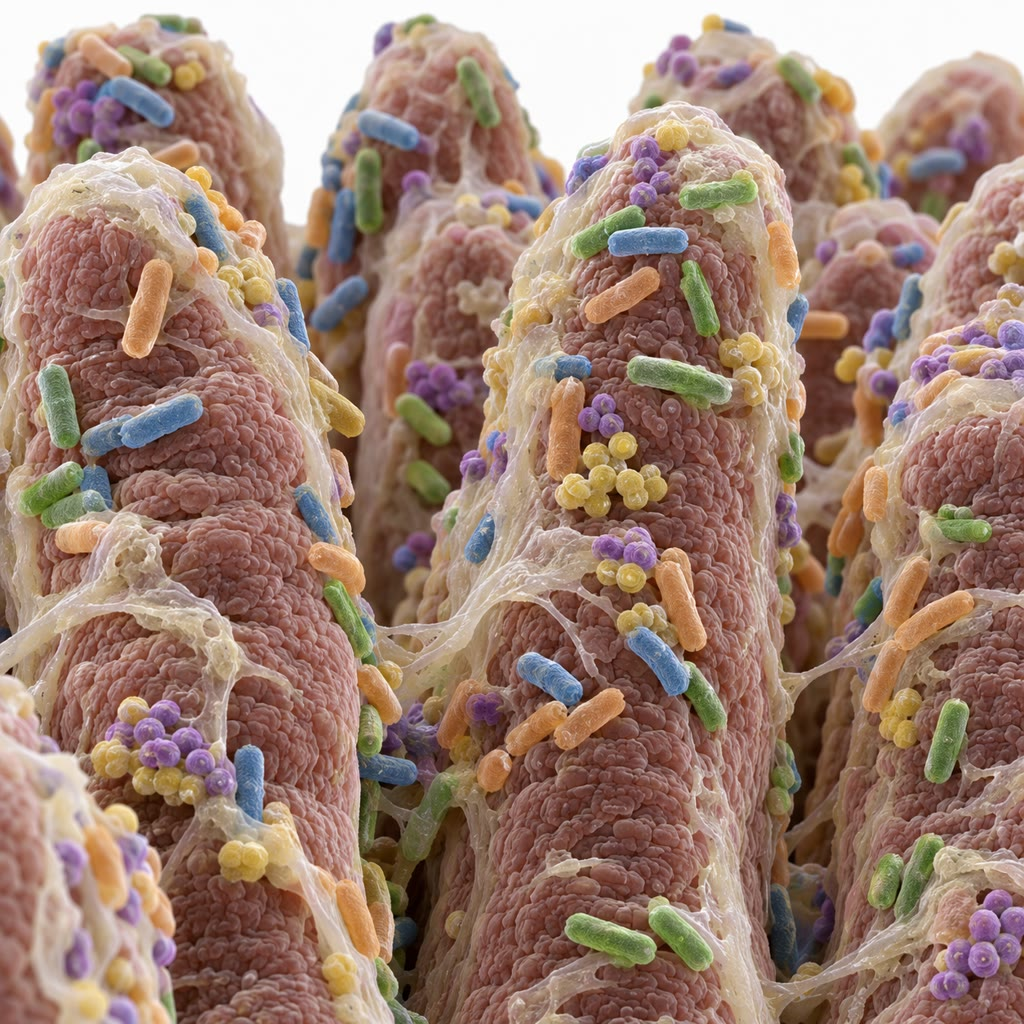
\includegraphics[width=0.40\linewidth]{images/book5/ai/b5-14-gut-microbiota.jpg}

{\small क्रमवीक्षण इलेक्ट्रॉन सूक्ष्मदर्शी में आंत्र-अस्तर का पृष्ठ,
जिसमें कई तरह के जीवाणु रसांकुरों के बीच की श्लेष्मा में जमे हैं।}
\end{omfigure}

\section{पौधे और उनके साथी}

\begin{definition}[शिंबी--राइजोबियम सहजीविता]\label{def:b3:microbiomes:nodule}
\index{राइजोबिया}\index{मूल-ग्रंथिका}\index{नॉड कारक}\index{लेग्हीमोग्लोबिन}\index{नाइट्रोजनेज़}
शिंबी पौधे नाइट्रोजन-स्थिरीकारी जीवाणु (\emph{राइजोबिया})
\emph{मूल-ग्रंथिकाओं} में रखते हैं, जो किसी आणविक संवाद के बाद इसी काम
के लिए बनाए गए अंग हैं। जड़ फ्लैवोनॉइड स्रवित करती है; मेल खाती जाति का
कोई राइजोबियम \emph{नॉड कारकों} से उत्तर देता है --- ऐसे
लिपोकाइटोऑलिगोसैकेराइड जिनकी सजावट साथी को निर्दिष्ट करती है; मूलरोम पर
बैठी कोई ग्राही काइनेज़ उन्हें बाँधती है और केंद्रक में कैल्सियम के
दोलन, जीवाणुओं के चारों ओर मूलरोम का कुंडलन, तथा कोई
\emph{संक्रमण-सूत्र} छेड़ देती है, जो कोशिकाओं से होकर भीतर की ओर बढ़ता
है जबकि नीचे का वल्कुट बँटकर ग्रंथिका बनने लगता है। जीवाणु झिल्लियों के
भीतर ग्रंथिका-कोशिकाओं में छोड़ दिए जाते हैं और \emph{बैक्टेरॉइडों} में
विभेदित होते हैं, जो \emph{नाइट्रोजनेज़} अभिव्यक्त करते हैं, यानी वह
एंज़ाइम जो प्रति अणु सोलह ATP की लागत पर N$_{2}$ को अमोनिया में अपचयित
करती है। नाइट्रोजनेज़ ऑक्सीजन से नष्ट हो जाती है, फिर भी बैक्टेरॉइड
ज़ोर से श्वसन करते हैं; ग्रंथिका इस विरोधाभास को किसी विसरण-अवरोध से और
\emph{लेग्हीमोग्लोबिन} से सुलझाती है, यानी किसी ऐसे पादप हीमोग्लोबिन से
जो ऑक्सीजन को कसकर बाँधता है और उसे किसी कम मुक्त सांद्रता पर
बैक्टेरॉइडों तक ढोता है --- वही किसी कटी ग्रंथिका को गुलाबी बनाता है।
पौधा अपने प्रकाश-संश्लेषित पदार्थ का छह से दस प्रतिशत चुकाता है और अपनी
अधिकांश नाइट्रोजन पाता है; संसार की शिंबी फ़सलों की स्थिर की गई
नाइट्रोजन उर्वरक-उद्योग की नाइट्रोजन के पास पहुँचती है।
\end{definition}

\begin{omfigure}
\begin{tikzpicture}[every node/.style={font=\scriptsize}, >=stealth]
  % stage 1: root hair and bacteria, flavonoid / Nod factor exchange
  \begin{scope}
    \draw[thick, omMeth!60!black, fill=omMeth!15] (0,0) rectangle (1.2,3.0);
    \draw[thick, omMeth!60!black, fill=omMeth!15] (1.2,1.6) .. controls (2.4,1.7) and (2.6,2.6) .. (2.9,2.4) .. controls (2.5,2.3) and (2.3,1.4) .. (1.2,1.2) -- cycle;
    \foreach \p in {(3.1,2.7),(3.4,2.3),(3.3,1.9)} \fill[omProp] \p ellipse (0.14 and 0.07);
    \draw[->, omMeth!60!black, thick] (2.6,1.5) -- (3.2,1.4); \node[below, omMeth!60!black] at (3.0,1.35) {फ्लैवोनॉइड};
    \draw[<-, omProp, thick] (2.5,2.85) -- (3.0,3.0); \node[above, omProp] at (2.4,2.95) {नॉड कारक};
    \node[below, align=center] at (1.6,-0.2) {1. संवाद: मूलरोम\\और राइजोबिया};
  \end{scope}
  % stage 2: curled hair, infection thread
  \begin{scope}[xshift=4.6cm]
    \draw[thick, omMeth!60!black, fill=omMeth!15] (0,0) rectangle (1.2,3.0);
    \draw[thick, omMeth!60!black, fill=omMeth!15] (1.2,1.6) .. controls (2.3,1.8) and (2.8,2.6) .. (2.2,2.8) .. controls (1.9,2.9) and (1.8,2.5) .. (2.0,2.4) .. controls (2.3,2.2) and (1.9,1.3) .. (1.2,1.2) -- cycle;
    \draw[omProp, very thick] (2.05,2.55) .. controls (1.8,2.1) and (1.4,1.7) .. (0.4,1.3);
    \foreach \p in {(1.85,2.3),(1.5,1.9),(1.1,1.6),(0.7,1.4)} \fill[omProp] \p ellipse (0.1 and 0.05);
    \node[right, omProp, font=\tiny] at (2.3,1.0) {संक्रमण-सूत्र};
    \foreach \p in {(0.3,0.5),(0.6,0.7),(0.9,0.5)} \draw[omMeth!60!black] \p circle (0.12);
    \node[below, align=center] at (1.6,-0.2) {2. रोम कुंडलित; सूत्र भीतर बढ़ता;\\वल्कुट कोशिकाएँ बँटतीं};
  \end{scope}
  % stage 3: nodule
  \begin{scope}[xshift=9.0cm]
    \draw[thick, omMeth!60!black, fill=omMeth!15] (0,0) rectangle (1.2,3.0);
    \draw[thick, omThm!60!black, fill=omThm!25] (1.2,1.5) ellipse (1.3 and 1.0);
    \foreach \p in {(1.0,1.5),(1.5,1.8),(1.6,1.2),(1.1,1.9),(1.2,1.1),(2.0,1.5)} \fill[omProp] \p circle (0.1);
    \node[right, align=left] at (2.6,2.0) {ग्रंथिका: नाइट्रोजनेज़ वाले\\बैक्टेरॉइड};
    \node[right, align=left, omThm!60!black] at (2.6,1.1) {गुलाबी: लेग्हीमोग्लोबिन\\O$_2$ कम रखता है};
    \draw[->, thick] (0.6,2.4) -- (1.0,2.0) node[pos=0, above] {शर्करा};
    \draw[<-, thick] (0.6,0.6) -- (1.0,1.0) node[pos=0, below] {NH$_3$};
    \node[below, align=center] at (1.6,-0.2) {3. बैक्टेरॉइड N$_2$ स्थिर करते;\\अमोनिया के बदले शर्करा};
  \end{scope}
\end{tikzpicture}

{\small कोई ग्रंथिका बनाना। जड़ से फ्लैवोनॉइड और राइजोबियम से \omterm{def:b3:microbiomes:nodule}{नॉड कारक}
साथियों की पहचान करा देते हैं; मूलरोम कुंडलित होता है, कोई
संक्रमण-सूत्र जीवाणुओं को भीतर ले जाता है, और वल्कुट कोई ऐसी ग्रंथिका
बनाता है जिसमें \omterm{def:b3:microbiomes:nodule}{लेग्हीमोग्लोबिन} से कम ऑक्सीजन पर रखे बैक्टेरॉइड शर्करा
के बदले नाइट्रोजन स्थिर करते हैं।}
\end{omfigure}

\begin{definition}[कवकमूल]\label{def:b3:microbiomes:mycorrhiza}
\index{कवकमूल}\index{अर्बुस्कुली कवकमूल}\index{साझा सहजीविता-पथ}
\emph{कवकमूल} जड़ों का कवकों के साथ साहचर्य है, जो पादप जातियों के कोई
\qty{80}{\%} में और थलीय पौधों के आरंभतम जीवाश्मों में मिलता है।
\emph{अर्बुस्कुली कवकमूलों} में कवक (कोई ग्लोमेरोमाइसीट) जड़ की
कोशिकाओं में घुसता है और किसी वृक्ष-सरीखे अर्बुस्कुल में शाखित होता है,
जिसके आर-पार फ़ॉस्फ़ेट, नाइट्रोजन और जल पौधे तक तथा शर्कराएँ और लिपिड
कवक तक जाते हैं; कवक-तंतु जड़ के अवशोषक पृष्ठ को सौ गुना बढ़ा देते हैं
और उस फ़ॉस्फ़ेट तक पहुँचते हैं जहाँ जड़ नहीं पहुँच सकती। वन-वृक्षों के
\emph{बाह्यकवकमूलों} में कवक जड़ को खोल की तरह ढँकता है और कोशिकाओं के
बीच बढ़ता है। पौधे के जो जीन कवक को भीतर आने देते हैं वे वही
\emph{साझा सहजीविता-पथ} हैं --- ग्राही, कैल्सियम की स्पंदमाला, अनुलेखन
कारक --- जिन्हें शिंबी पौधे \omterm{def:b3:microbiomes:nodule}{राइजोबिया} के लिए फिर काम में लेते हैं:
ग्रंथिका कोई देर की ईजाद है, जो अपने से चालीस करोड़ वर्ष पुरानी किसी
कवक-साझेदारी पर बनी है।
\end{definition}

\begin{proposition}[व्यापार और उसकी चौकसी]\label{prop:b3:microbiomes:sanctions}
\index{साथी-चयन}\index{प्रतिबंध}\index{छली}
कोई \omterm{def:b3:microbiomes:symbiosis}{सहोपकारिता} एक विनिमय है, और हर साथी कम देने तथा अधिक लेने के लिए
चुना जाता है; वह इसलिए टिकती है कि दूसरा साथी पलटवार कर सकता है। शिंबी
पौधे उन ग्रंथिकाओं की ऑक्सीजन रोक देते हैं जिनके \omterm{def:b3:microbiomes:nodule}{राइजोबिया} नाइट्रोजन
नहीं स्थिर करते, और उनका जनन आधा कर देते हैं (कीयर्स, 2003): यही
\emph{प्रतिबंध} हैं। कवकमूली जालों में पौधे उन कवक-साथियों को अधिक
कार्बन देते हैं जो अधिक फ़ॉस्फ़ेट पहुँचाते हैं, और कवक उन जड़ों को अधिक
फ़ॉस्फ़ेट जो अधिक कार्बन चुकाती हैं --- कोई बाज़ार, जिसमें दोनों पक्ष
बेहतर व्यापारी को पुरस्कृत करते हैं (कीयर्स, 2011)। स्क्विड
प्रकाश-अंग के उन जीवाणुओं को बाहर कर देते हैं जो चमकते नहीं; मनुष्यों
के प्रतिरक्षा-तंत्र उन सहभोजियों को सहते हैं जो अवकाशिका में रहते हैं
और उन पर वार करते हैं जो दीवार पार करते हैं। जहाँ कोई परपोषी न चुन
सकता है न प्रतिबंध लगा सकता --- कोई अंतःसहजीवी जो अंडे से विरासत में
मिले --- वहाँ हितों का मेल इसके बजाय साझा नियति से आता है: ऊर्ध्वाधर
रूप से संचरित कोई सहजीवी तभी जनन करता है जब उसका परपोषी करे, और सहजीवी
पर वरण परपोषी के जनन के पक्ष में होता है। इस तरह संचरण की रीति
साझेदारी का चरित्र बता देती है: \omterm{def:b3:microbiomes:symbiosis}{ऊर्ध्वाधर संचरण} \omterm{def:b3:microbiomes:symbiosis}{सहोपकारिता} और निर्भरता
की ओर, क्षैतिज संचरण उस दोहन की ओर जिसे चौकसी काबू में रखती है।
\end{proposition}
\admitted

\begin{omfigure}
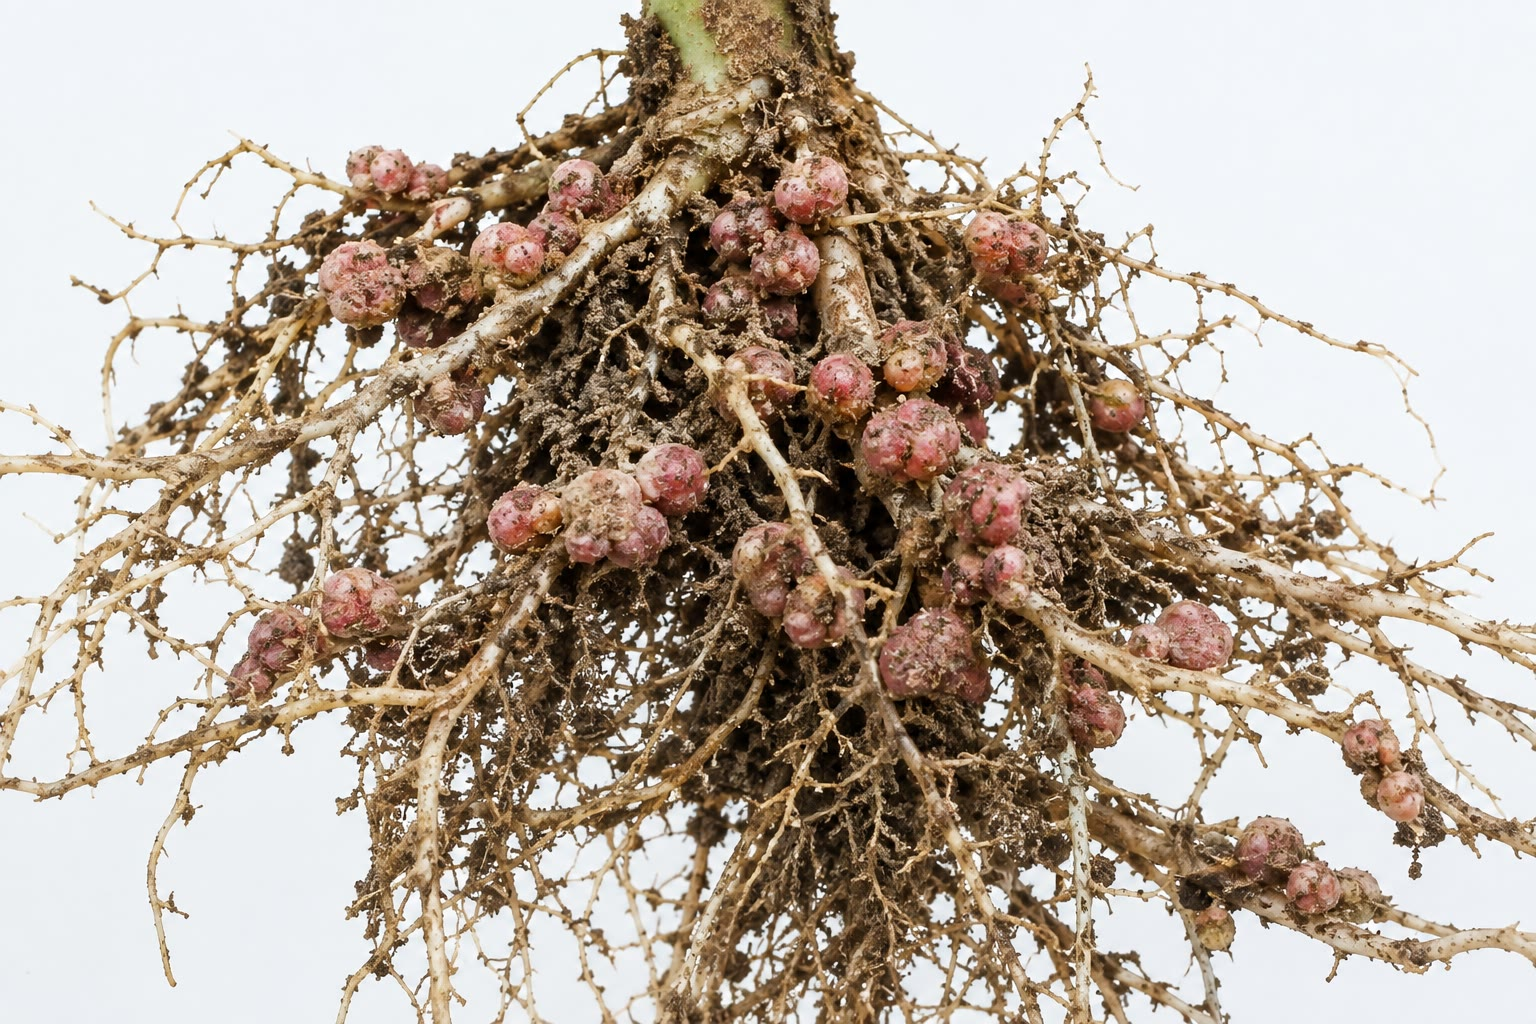
\includegraphics[width=0.46\linewidth]{images/book5/ai/b5-14-root-nodules.jpg}\hspace{0.04\linewidth}
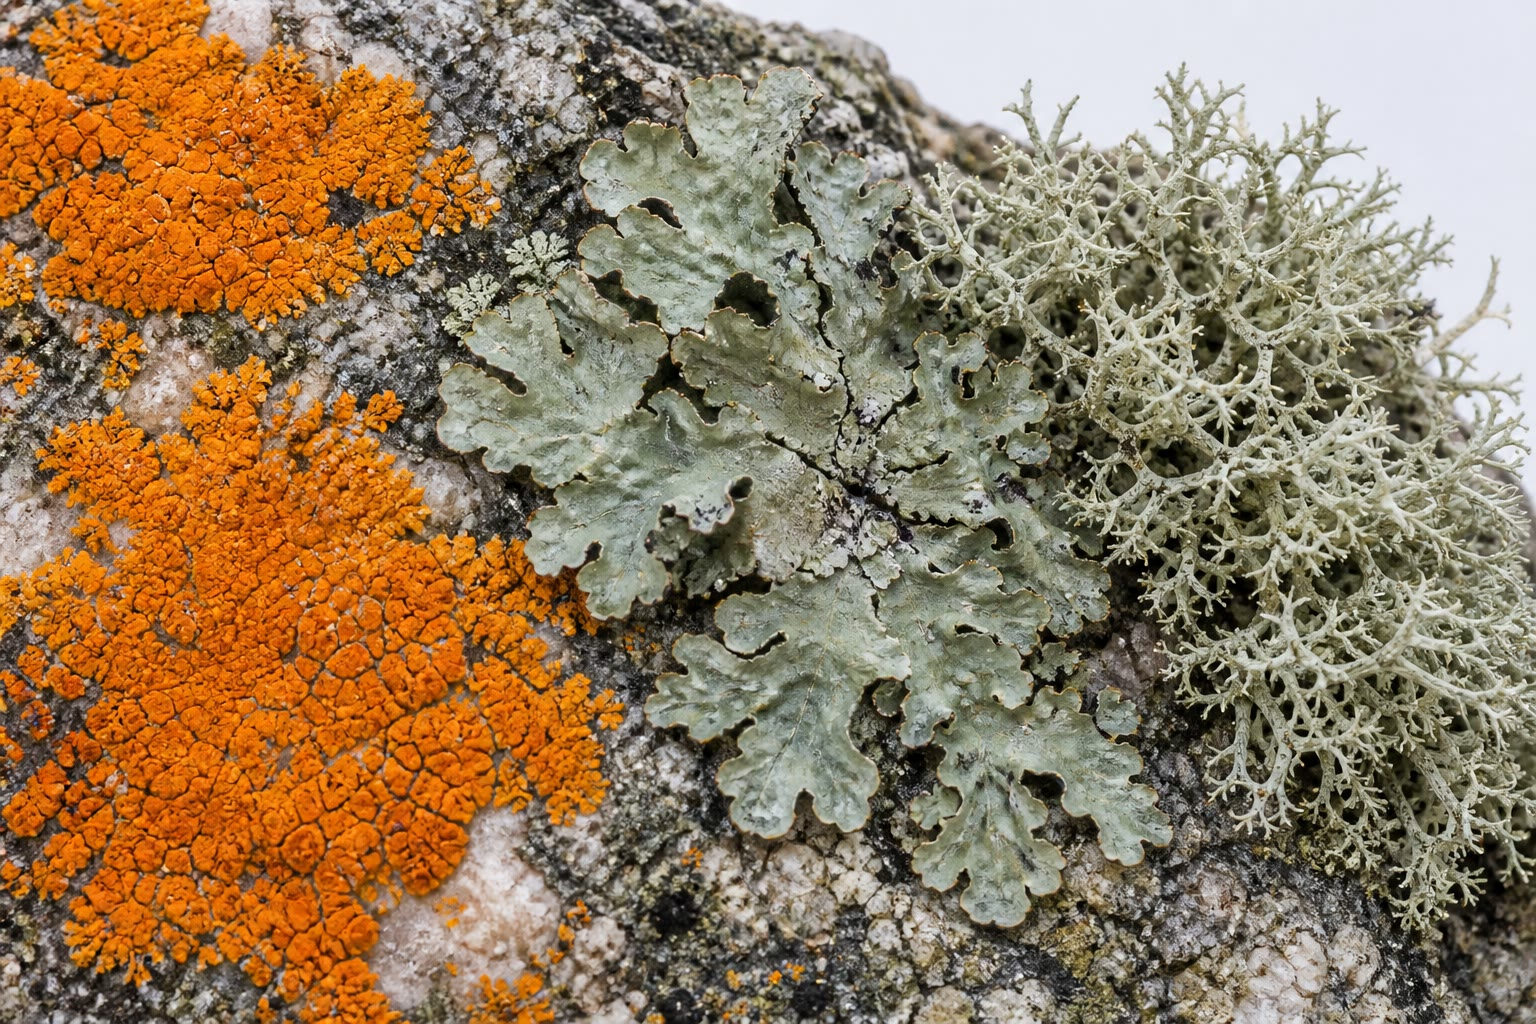
\includegraphics[width=0.46\linewidth]{images/book5/ai/b5-14-lichen.jpg}

{\small बाएँ: किसी शिंबी पौधे की ग्रंथिकाओं वाली जड़ें, हर गुलाबी
ग्रंथिका शर्करा से पोषित बैक्टेरॉइडों का कोई नाइट्रोजन-कारखाना। दाएँ:
चट्टान पर लाइकेन --- हर एक कोई कवक, जो किसी प्रकाश-संश्लेषी शैवाल या
सायनोजीवाणु को बसाए है, और दोनों मिलकर ऐसा पृष्ठ बसा लेते हैं जिसे
अकेला कोई थाम नहीं सकता था।}
\end{omfigure}

\section{समुद्र में और अन्यत्र साझेदारियाँ}

\begin{definition}[प्रवाल और शैवाल]\label{def:b3:microbiomes:coral}
\index{प्रवाल सहजीविता}\index{ज़ूज़ैंथेली}\index{प्रवाल-विवर्णन}
रीफ़ बनाते प्रवाल अपनी आंत्र-अस्तर की कोशिकाओं के भीतर डाइनोफ़्लैजलेट
शैवाल (\emph{Symbiodiniaceae}, यानी \emph{ज़ूज़ैंथेली}) रखते हैं, प्रति
वर्ग सेंटीमीटर दस लाख या उससे अधिक। ये शैवाल प्राणी के ऊतक में, प्राणी
के अपशिष्ट CO$_{2}$, अमोनिया और फ़ॉस्फ़ेट से प्रकाश-संश्लेषण करते हैं,
और अपने स्थिर किए कार्बन का \qty{90}{\%} तक ग्लिसरॉल, शर्कराओं और
ऐमीनो अम्लों के रूप में लौटा देते हैं, जो प्रवाल को और उस कैल्सीभवन को
खिलाते हैं जो रीफ़ बनाता है; बदले में प्रवाल शैवालों की
नाइट्रोजन-पूर्ति और इसलिए उनकी वृद्धि पर काबू रखता है। यह साझेदारी किसी
सँकरी तापीय खिड़की के भीतर ही चलती है: जब जल ग्रीष्म के अधिकतम से कोई
एक-दो अंश ऊपर कुछ सप्ताह बना रहे, तब शैवालों का प्रकाश-संश्लेषण
क्षतिग्रस्त होता है, वे परपोषी कोशिकाओं में क्रियाशील ऑक्सीजन छोड़ते
हैं, और प्रवाल उन्हें बाहर कर देता है --- यही \emph{विवर्णन} है, जिसमें
पारभासी प्राणी के आर-पार सफ़ेद कंकाल दिखने लगता है। विवर्णित प्रवाल भूखा
मरता है; यदि जल सप्ताहों के भीतर ठंडा हो जाए तो वह सँभल जाता है, नहीं
तो मर जाता है। विवर्णन की बारंबारता 1980 से पाँच गुना बढ़ी है, और यही
वह तंत्र है जिससे तापन रीफ़ों को मिटा रहा है।
\end{definition}

\begin{example}[आवास बनाती सहजीविताएँ]\label{ex:b3:microbiomes:habitats}
कोई \emph{लाइकेन} ऐसा कवक है जो किसी हरे शैवाल या किसी सायनोजीवाणु को
बसाए रखता है; कवक संरचना, जल-धारण और चट्टान से घुले खनिज देता है, और
प्रकाशजीवी शर्करा (और यदि वह सायनोजीवाणु हो तो नाइट्रोजन भी)। लाइकेन
थल-पृष्ठ के कोई \qty{8}{\%} ढँकते हैं, नंगी चट्टान पर बसते हैं, और
उसका मिट्टी में बदलना शुरू करते हैं। गहरे समुद्र के उद्गारों का
नलिका-कृमि \emph{Riftia} वयस्क होने पर न मुँह रखता है न आँत; वह किसी
ट्रोफ़ोसोम में सल्फ़ाइड-ऑक्सीकारी जीवाणु बसाता है और उन्हें सल्फ़ाइड तथा
ऑक्सीजन किसी ऐसे हीमोग्लोबिन पर पहुँचाता है जो दोनों बाँधता है, और
अँधेरे में रासायनिक ऊर्जा पर साल में एक मीटर से अधिक बढ़ता है। दीमक
लकड़ी को आद्यजीवों और जीवाणुओं के किसी आँत-समुदाय से पचाते हैं, और
रोमंथी घास को किसी ऐसे रूमेन से, जो नहाने के टब जितना बड़ा है और जिसमें
जीवाणु, आर्किया तथा कवक सेलुलोस को वसा अम्लों और मेथैन में किण्वित करते
हैं; गाय उन्हीं वसा अम्लों पर और स्वयं उन सूक्ष्मजीवों के शरीरों पर
जीती है। हर स्थिति में कोई उपापचयी सामर्थ्य --- प्रकाश-संश्लेषण,
नाइट्रोजन-स्थिरीकरण, सल्फ़ाइड-ऑक्सीकरण, सेलुलोस-पाचन --- जो परपोषी की
वंश-परंपरा ने कभी विकसित नहीं किया, साझेदारी से एक ही कदम में पा लिया
गया है।
\end{example}

\begin{omfigure}
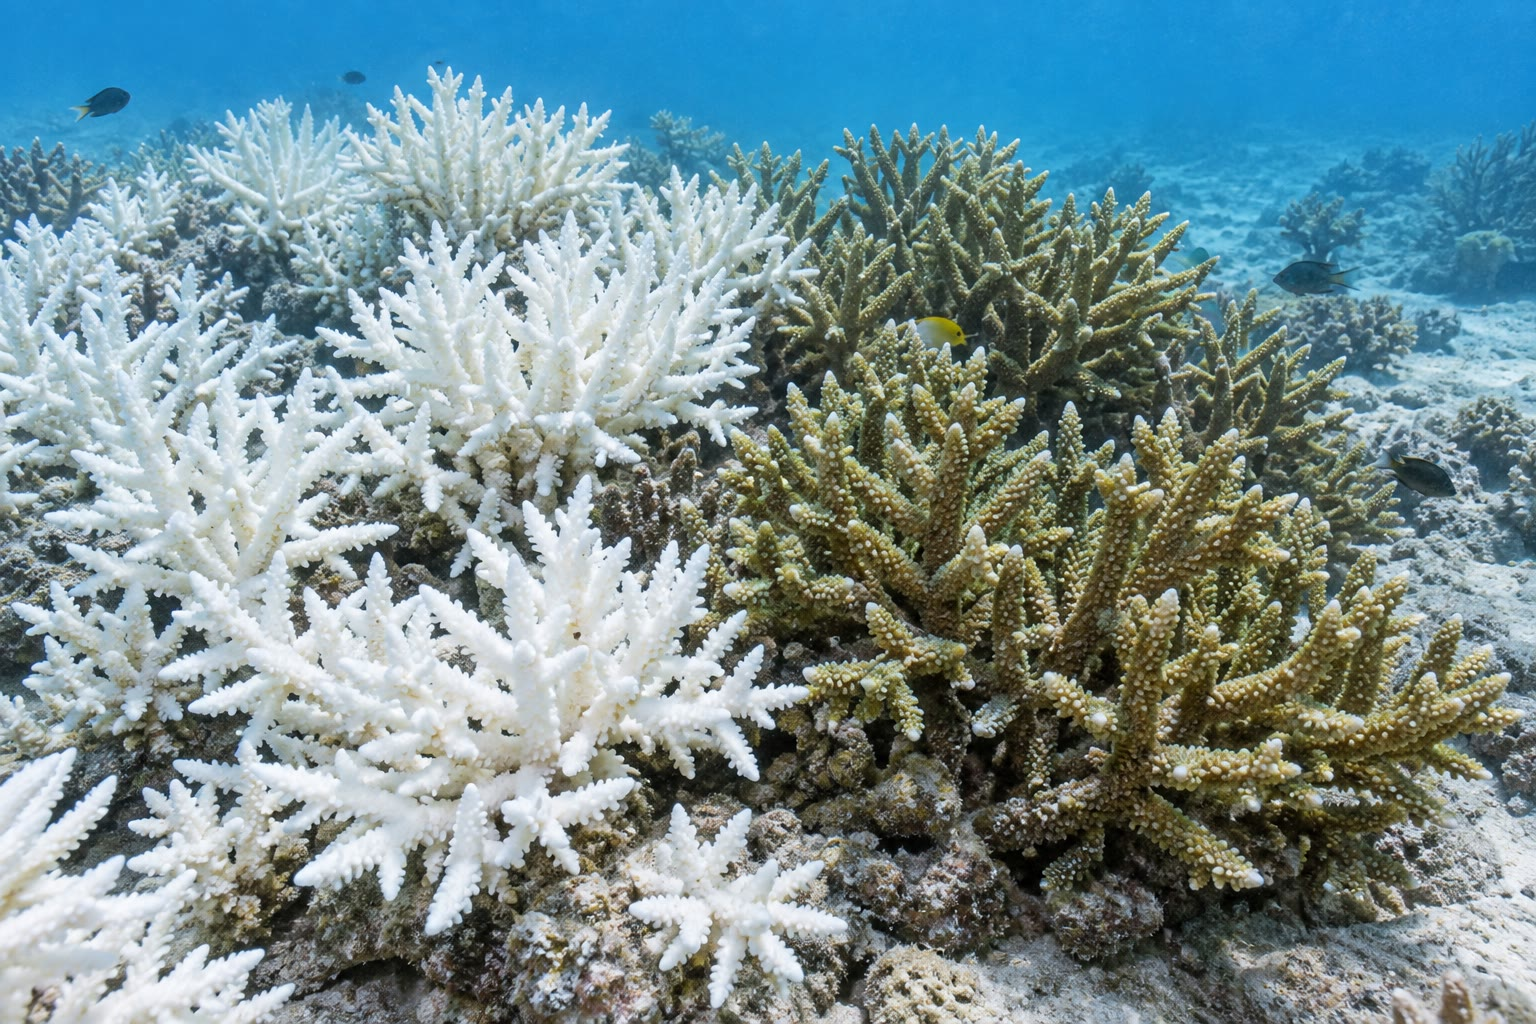
\includegraphics[width=0.56\linewidth]{images/book5/ai/b5-14-coral-bleaching.jpg}

{\small आधी विवर्णित कोई रीफ़: सफ़ेद बस्तियाँ हफ़्तों के अति गरम जल के
बाद अपने शैवाल बाहर कर चुकी हैं; भूरी अब भी अपने थामे हैं। सफ़ेद प्रवाल
जीवित और भूखा है, और उसके पास फिर बसाए जाने के लिए कुछ हफ़्ते हैं।}
\end{omfigure}

\begin{omfigure}
\begin{tikzpicture}[every node/.style={font=\scriptsize}, >=stealth]
  % coral cell with alga
  \draw[very thick, omDef, fill=omDef!8] (0,0) ellipse (3.2 and 2.0); \node[above] at (0,2.05) {प्रवाल कोशिका (जठरचर्म)};
  \draw[thick, omMeth!70!black, fill=omMeth!30] (-0.4,-0.1) circle (1.05); \node[align=center] at (-0.4,-0.1) {शैवाल\\(ज़ूज़ैंथेला)};
  % exchanges
  \draw[->, thick, omMeth!70!black] (0.5,0.4) -- (1.9,0.9) node[right, align=left] {ग्लिसरॉल, शर्कराएँ, ऐमीनो अम्ल:\\स्थिर किए कार्बन का \qty{90}{\%} तक};
  \draw[<-, thick, omThm] (0.5,-0.5) -- (1.9,-1.0) node[right, align=left] {CO$_2$, NH$_3$, फ़ॉस्फ़ेट\\(प्राणी के अपशिष्ट)};
  \draw[<-, thick, omProp] (-1.3,0.3) -- (-2.6,1.0) node[left, align=right] {ऊतक से होकर\\आता प्रकाश};
  \node[below, align=center] at (1.5,-2.1) {दबाव: हफ़्तों तक गरम जल $\to$ प्रकाश-संश्लेषण क्षतिग्रस्त,\\क्रियाशील ऑक्सीजन $\to$ शैवाल बाहर $\to$ विवर्णन};
  % thermometer-like bar on the right
  \begin{scope}[xshift=7.6cm, yshift=-1.6cm]
    \draw[thick] (0,0) rectangle (0.5,3.2);
    \fill[omDef!40] (0,0) rectangle (0.5,2.0); \fill[omProp!60] (0,2.0) rectangle (0.5,2.6); \fill[omThm!60] (0,2.6) rectangle (0.5,3.2);
    \node[right] at (0.6,1.0) {सामान्य परास}; \node[right] at (0.6,2.3) {$+\qty{1}{\celsius}$: दबाव}; \node[right, align=left] at (0.6,2.9) {हफ़्तों तक $+\qty{2}{\celsius}$:\\विवर्णन};
    \node[below, align=center] at (0.25,-0.1) {ग्रीष्म का समुद्री\\तापमान};
  \end{scope}
\end{tikzpicture}

{\small प्रवाल--शैवाल विनिमय: शैवाल प्राणी के अपशिष्टों और उसके ऊतक से
आते प्रकाश से कार्बन स्थिर करता है और उसका अधिकांश भोजन के रूप में
लौटा देता है; तापमान की छोटी, टिकाऊ बढ़त इस साझेदारी को तोड़ देती है।}
\end{omfigure}

\section{साथी से कोशिकांग तक}

\begin{proposition}[जीनोम-संकुचन और कोशिकांग तक की राह]\label{prop:b3:microbiomes:reduction}
\index{जीनोम-संकुचन}\index{अंतःसहजीवी जीन-अंतरण}
अंडे से विरासत में मिला कोई अंतःसहजीवी कुछ ही कोशिकाओं की उस समष्टि में
रहता है जो बाहरवालों के साथ कभी पुनर्संयोजन नहीं करती। उस पर वरण कमज़ोर
है (\cref{ch:b3:molecular-evolution}: कोई छोटी समष्टि थोड़े हानिकारक
उत्परिवर्तन अपवाह से स्थिर कर देती है), जिन जीनों के उत्पाद परपोषी
जुटाता है वे टूटने पर खटकते नहीं, और खोया जीन कभी वापस नहीं मिलता।
इसलिए जीनोम पीढ़ी-दर-पीढ़ी सिकुड़ता जाता है --- \emph{Buchnera}
\qty{640}{kb} तक, कुछ कीट-सहजीवी \qty{140}{kb} और कुछ सौ जीनों तक,
मनुष्यों में सूत्रकणिका \qty{16}{kb} और तेरह प्रोटीनों तक --- और
परपोषी का केंद्रक \emph{\omterm{prop:b3:microbiomes:reduction}{अंतःसहजीवी जीन-अंतरण}} से सहजीवी जीनों की
प्रतियाँ पा लेता है, जिनके उत्पाद किसी लक्ष्यन-अनुक्रम के साथ वापस
आयातित होते हैं। जब परपोषी सहजीवी के अधिकांश प्रोटीन बनाने लगे, उसके
विभाजन पर काबू रखे, और उसके बिना जी न सके, तब सहजीवी कोशिकांग बन चुका
होता है। सूत्रकणिकाओं और लवकों ने यह राह दो अरब और एक अरब वर्ष पहले
तय की (वर्ष~1 का खंड); \emph{Paulinella} का वर्णलवक तीसरा राही है, जो
दस करोड़ वर्ष चल चुका है।
\end{proposition}

\begin{remark}[व्यष्टि पर फिर से]\label{rem:b3:microbiomes:individual}
कोई प्राणी या पौधा अपने केंद्र में किसी जीनोम के साथ एक समुदाय है,
जिसके उपापचयी भंडार का अधिकांश, और जिसके परिवर्धन तथा प्रतिरक्षा का
बहुत कुछ, उन साथियों पर टिका है जो उसे अपने ही DNA में विरासत में नहीं
मिले। व्यावहारिक परिणाम अभी से यहाँ हैं: \omterm{def:b3:microbiomes:symbiosis}{माइक्रोबायोम} किसी औषध के रूप
में (मल-प्रत्यारोपण), औषधों के लक्ष्य के रूप में (\omterm{def:b3:bacteriology:antibiotics}{प्रतिजैविकों} की
पार्श्व-क्षति, नुस्खे के रूप में आहारीय रेशा), किसी निदान-साधन के रूप
में, और --- अभियंत्रित सहजीवियों तथा \emph{Wolbachia} ढोते मच्छरों के
ज़रिए --- जंगली समष्टियों का जीव-विज्ञान बदलने के रास्ते के रूप में।
सैद्धांतिक परिणाम यह है कि प्राकृतिक वरण साझेदारियों पर काम करता है,
और सबसे मज़बूत साझेदारियाँ वे हैं जिनमें एक साथी की नियति दूसरे की
नियति है।
\end{remark}

\section{अभ्यास}

\begin{exercise}[$\star$]\label{exo:b3:microbiomes:1}
\omterm{def:b3:microbiomes:symbiosis}{सहोपकारिता}, \omterm{def:b3:microbiomes:symbiosis}{सहभोजिता} और परजीविता को परिभाषित कीजिए, और इस अध्याय से हर
एक का एक-एक उदाहरण दीजिए। जातियों की एक ही जोड़ी इन कोटियों के बीच
क्यों सरक सकती है?
\end{exercise}

\begin{exercise}[$\star$]\label{exo:b3:microbiomes:2}
किसी ऐसे समुदाय के लिए $H$, $e^{H}$, $D$ और $1/D$ निकालिए जिसकी
प्रचुरताएँ $0.5$, $0.3$, $0.1$, $0.05$, $0.05$ हों।
\end{exercise}

\begin{exercise}[$\star$]\label{exo:b3:microbiomes:3}
किसी 16S ऐम्प्लिकॉन सर्वेक्षण और शॉटगन मेटाजीनोमिकी की तुलना कीजिए:
हर एक क्या बताती है, और हर एक आपको क्या नहीं बता सकती?
\end{exercise}

\begin{exercise}[$\star$]\label{exo:b3:microbiomes:4}
\omterm{def:b3:microbiomes:gut}{आँत का माइक्रोबायोम} अपने परपोषी को जो चार सेवाएँ देता है वे गिनाइए, और
उसके बिगड़ने से होने वाला एक रोग बताइए।
\end{exercise}

\begin{exercise}[$\star\star$]\label{exo:b3:microbiomes:5}
$N = 20$ \omterm{def:b3:genomics:ngs}{वाचनों} के किसी प्रतिदर्श में ऐसी जातियाँ हैं जिनके $N_{i} = 10, 6, 3, 1$ हैं।
प्रमेय से $E[S_{n}]$ को $n = 5$ के लिए निकालिए, और \omterm{thm:b3:microbiomes:rarefaction}{गुड का आच्छादन} भी।
\end{exercise}

\begin{exercise}[$\star\star$]\label{exo:b3:microbiomes:6}
बृहदांत्र में \qty{400}{g} अंतर्वस्तु है, प्रति ग्राम $10^{11}$
जीवाणु; किसी जीवाणु का भार \qty{1}{pg} है और उसके जीनोम में \num{4000}
जीन; किसी व्यक्ति की आँत में $1000$ जातियाँ हैं। \omterm{def:b3:microbiomes:symbiosis}{माइक्रोबायोम} का
द्रव्यमान और उसके ढोए भिन्न जीनों की संख्या आँकिए, और मानव जीनोम के
\num{20000} से तुलना कीजिए।
\end{exercise}

\begin{exercise}[$\star\star$]\label{exo:b3:microbiomes:7}
ग्रंथिका का ऑक्सीजन-विरोधाभास समझाइए, और यह भी कि \omterm{def:b3:microbiomes:nodule}{लेग्हीमोग्लोबिन} तथा
विसरण-अवरोध उसे कैसे सुलझाते हैं। कोई ग्रंथिका गुलाबी क्यों होती है,
और हरी ग्रंथिका का क्या अर्थ है?
\end{exercise}

\begin{exercise}[$\star\star$]\label{exo:b3:microbiomes:8}
किसी शिंबी उत्परिवर्ती में \omterm{def:b3:microbiomes:mycorrhiza}{साझा सहजीविता-पथ} का कैल्सियम-स्पंदन घटक नहीं
है। उसके ग्रंथिकन और उसके कवकमूलन का पूर्वानुमान कीजिए, और समझाइए कि
इससे दोनों \omterm{def:b3:microbiomes:symbiosis}{सहजीविताओं} के विकास के बारे में क्या पता चलता है।
\end{exercise}

\begin{exercise}[$\star\star$]\label{exo:b3:microbiomes:9}
कीयर्स के प्रतिबंध-प्रयोग का वर्णन कीजिए, और यह भी कि यदि पौधा
स्थिरीकारी और अस्थिरीकारी ग्रंथिकाओं में भेद न कर पाता तो क्या होता।
\end{exercise}

\begin{exercise}[$\star\star\star$]\label{exo:b3:microbiomes:10}
सिद्ध कीजिए कि \omterm{def:b3:microbiomes:diversity}{विरलन} प्रमेय का $E[S_{n}]$ $n$ का कोई वर्धमान फलन है और
$S$ तक पहुँचता है जब $n = N$, और दिखाइए कि $N_{i} \ll N$ तथा
$n \ll N$ वाली किसी जाति के देखे जाने की प्रायिकता लगभग
$1 - (1 - n/N)^{N_{i}}$ है।
\end{exercise}

\begin{exercise}[$\star\star\star$]\label{exo:b3:microbiomes:11}
\emph{Wolbachia} केवल अंडों से संचरित होता है। समझाइए कि उस पर वरण
मादा परपोषियों के पक्ष में क्यों होता है, कोशिकाद्रव्यी असंगति का
वर्णन कीजिए, और दिखाइए कि वह किसी संक्रमित प्रभेद को तब भी क्यों फैलने
देती है जब संक्रमण की कोई छोटी लागत हो।
\end{exercise}

\begin{exercise}[$\star\star\star$]\label{exo:b3:microbiomes:12}
\cref{prop:b3:microbiomes:reduction} का उपयोग करते हुए समझाइए कि
ऊर्ध्वाधर रूप से संचरित अंतःसहजीवियों के जीनोम क्यों सिकुड़ते हैं जबकि
उनके स्वतंत्र-जीवी नातेदारों के नहीं, कौन-से जीन पहले खोए जाते हैं और
कौन-से आख़िर में, और इस प्रवृत्ति को क्या उलटेगा।
\end{exercise}

\section{समस्या: किसी आँत की जनगणना}

\begin{problem}[{सप्तांत समस्या --- कोई आँत का माइक्रोबायोम कोशिकाओं,
जीनों और कैलोरियों में गिना गया, उसकी विविधता नापी और विरल की गई, किसी
शिंबी का नाइट्रोजन-बजट उसकी शर्करा के सामने तोला गया, और किसी रीफ़ का
कार्बन-लेखा किया गया, जिसका अंत उन कैलोरियों पर होता है जो कोई
माइक्रोबायोम कमाता है, किसी अनुक्रमण-प्रतिदर्श के आच्छादन पर, और उस
शर्करा पर जो सेम का कोई खेत अपनी नाइट्रोजन के लिए चुकाता है}]
\label{pb:b3:microbiomes:1}
आँकड़े: बृहदांत्र की अंतर्वस्तु \qty{400}{g}, प्रति ग्राम $10^{11}$
जीवाणु, कोशिका-द्रव्यमान \qty{1}{pg}; $1000$ जातियाँ, हर एक के
\num{4000} जीन, किन्हीं दो जातियों के बीच \qty{30}{\%} जीन साझा।
आहार: दिन में \qty{30}{g} रेशा, जो प्रति ग्राम \qty{10}{mmol} की दर से
\omterm{def:b3:microbiomes:gut}{लघु-शृंखला वसा अम्लों} में किण्वित होता है, हर एक \qty{0.9}{kJ} का;
आहार \qty{9000}{kJ} का। कोई अनुक्रमण-प्रतिदर्श: $N = 2000$ \omterm{def:b3:genomics:ngs}{वाचन},
$S = 180$ जातियाँ, $f_{1} = 60$ एकाकी; ऊपर की तीन जातियों की प्रचुरताएँ
$0.30$, $0.20$, $0.10$, बाकी बराबर फैली हुई। सेम की कोई फ़सल प्रति
हेक्टेयर प्रति मौसम \qty{150}{kg} N स्थिर करती है और स्थिर की गई प्रति
ग्राम N के लिए \qty{8}{g} शर्करा चुकाती है; उसका प्रकाश-संश्लेषण प्रति
हेक्टेयर प्रति मौसम \qty{12}{t} शर्करा देता है। \omterm{def:b3:microbiomes:nodule}{नाइट्रोजनेज़}: $16$ ATP
प्रति N$_{2}$। कोई प्रवाल: $10^{6}$ शैवाल प्रति cm$^{2}$, हर एक दिन
में \qty{20}{pg} कार्बन स्थिर करता है, जिसका \qty{90}{\%} परपोषी को
जाता है; प्रवाल-ऊतक \qty{15}{\micro g} कार्बन प्रति cm$^{2}$ प्रति दिन
श्वसित करता है।

\medskip
\noindent\textbf{भाग I --- कोशिकाएँ और जीन।}
\begin{enumerate}
  \item बृहदांत्र में कितने जीवाणु हैं, और उनका भार क्या है?
  \item वह कितने जीवाणु-जीनोमों जितना DNA है, और वह कुल
        $3\times 10^{13}$ मानव कोशिकाओं (हर एक \qty{6.4}{pg}) के DNA
        के सामने कैसा बैठता है?
  \item आँत में भिन्न जीवाणु-जीनों की संख्या आँकिए, \qty{30}{\%}
        अतिव्यापन को ध्यान में रखते हुए (हर जाति के असाझा \qty{70}{\%}
        जमा एक साझा समुच्चय गिनिए)। \num{20000} से तुलना कीजिए।
  \item वह रेशा प्रति दिन कितने मिलीमोल \omterm{def:b3:microbiomes:gut}{लघु-शृंखला वसा अम्ल} देता है,
        कितने किलोजूल, और आहार का कितना अंश?
  \item किसी रोगाणु-मुक्त चूहे को \qty{30}{\%} अधिक भोजन चाहिए। क्या
        प्रश्न 4 का वसा-अम्ल योगदान इसे समझाने के लिए पर्याप्त है? और
        क्या समझा सकता है?
  \item जीवाणु बृहदांत्र में लगभग दिन में एक बार बँटते हैं और
        अंतर्वस्तु उसी दर से निकल जाती है। इससे कौन-सी स्थायी अवस्था
        बनती है, और जब \omterm{def:b3:bacteriology:antibiotics}{प्रतिजैविकों} का कोई क्रम \qty{99.9}{\%}
        कोशिकाएँ मार दे तो उस समुदाय का क्या होता है?
\end{enumerate}

\medskip
\noindent\textbf{भाग II --- विविधता।}
\begin{enumerate}[resume]
  \item $177$ गौण जातियों में से हर एक की सापेक्ष प्रचुरता निकालिए,
        फिर \omterm{def:b3:microbiomes:diversity}{शैनन सूचकांक} $H$ और $e^{H}$।
  \item \omterm{def:b3:microbiomes:diversity}{सिम्पसन सूचकांक} $D$ और $1/D$ निकालिए। $1/D$ $e^{H}$ से छोटा
        क्यों है?
  \item प्रतिदर्श का गुड-आच्छादन; प्रति हज़ार कितने \omterm{def:b3:genomics:ngs}{वाचन} अनदेखी जातियों
        के हैं?
  \item उसी आँत से \num{10000} \omterm{def:b3:genomics:ngs}{वाचनों} का कोई दूसरा प्रतिदर्श $260$
        जातियाँ देता है। \omterm{def:b3:microbiomes:diversity}{विरलन} प्रमेय से समझाइए कि यह कोई विरोधाभास
        क्यों नहीं, और दोनों की तुलना से पहले क्या करना चाहिए।
  \item प्रमेय में, $N_{i} = 1$ वाली कोई जाति $n = 1000$ के किसी ऐसे
        उप-प्रतिदर्श में, जो $N =
        2000$ में से लिया गया हो, किस प्रायिकता से प्रकट होती है?
        $N_{i} = 5$ के साथ?
  \item \omterm{def:b3:bacteriology:antibiotics}{प्रतिजैविकों} के बाद वही आँत $60$ जातियाँ, $H = 2.0$, और एक
        जाति $0.5$ प्रचुरता पर दिखाती है। $e^{H}$ और $D$ निकालिए और उस
        समुदाय का शब्दों में वर्णन कीजिए।
\end{enumerate}

\medskip
\noindent\textbf{भाग III --- ग्रंथिका का लेखा।}
\begin{enumerate}[resume]
  \item फ़सल प्रति हेक्टेयर अपनी \qty{150}{kg} N के लिए कितनी शर्करा
        चुकाती है, और वह उसके प्रकाश-संश्लेषण का कितना अंश है?
  \item N$_{2}$ के कितने मोल \qty{150}{kg} N हैं, और \omterm{def:b3:microbiomes:nodule}{नाइट्रोजनेज़} उस
        पर ATP के कितने मोल खर्च करती है?
  \item श्वसित प्रति ग्लूकोस $30$ ATP पर, वह ATP कितने किलोग्राम
        ग्लूकोस के बराबर है? चुकाई गई शर्करा से तुलना कीजिए; बाकी
        किसलिए है?
  \item औद्योगिक अमोनिया की लागत प्रति kg N लगभग \qty{35}{MJ} है।
        प्रति ग्राम शर्करा \qty{16}{kJ} लेकर फ़सल की नाइट्रोजन की
        ऊर्जा-लागत की कारख़ाने से तुलना कीजिए।
  \item कोई अस्थिरीकारी राइजोबियम किसी ग्रंथिका में घुसता है। यदि पौधा
        उसकी ऑक्सीजन आधी करके उस पर प्रतिबंध लगाए और उसका जनन आधा रह
        जाए, तो अगले मौसम के \omterm{def:b3:microbiomes:nodule}{राइजोबिया} का कितना अंश छली होगा, यदि वे
        \qty{10}{\%} से शुरू हुए हों और स्थिरीकारी सामान्य जनन करें?
        (एक चक्र।)
  \item प्रतिबंधों के बिना, वे छली जो स्थिरीकरण की लागत बचाते हैं
        \qty{20}{\%} अधिक जनन करते हैं। उसी शुरुआत से, दस मौसमों में
        कितना अंश छली होगा? यह तुलना क्या दिखाती है?
\end{enumerate}

\medskip
\noindent\textbf{भाग IV --- रीफ़ का लेखा।}
\begin{enumerate}[resume]
  \item एक वर्ग सेंटीमीटर के शैवाल प्रति दिन कितना कार्बन स्थिर करते
        हैं, और कितना प्रवाल तक पहुँचता है?
  \item प्रवाल के श्वसन से तुलना कीजिए। अधिशेष क्या है, और वह किस काम
        आता है?
  \item विवर्णन के बाद \qty{95}{\%} शैवाल जा चुके हैं। जुटाया गया
        कार्बन फिर से निकालिए। \qty{300}{\micro g} कार्बन प्रति
        cm$^{2}$ के भंडार पर प्रवाल कितनी देर टिक सकता है?
  \item दबाव प्रायः डिग्री-ताप-सप्ताहों में नापा जाता है: मौसम भर में
        ग्रीष्म के अधिकतम से ऊपर की साप्ताहिक अधिकता का योग।
        $+\qty{1}{\celsius}$ पर आठ सप्ताह या $+\qty{2}{\celsius}$ पर
        चार, दोनों $8$ देते हैं; विवर्णन $4$ के पास शुरू होता है।
        दोनों में से कौन-सी रूपरेखा अधिक बुरी है, और फिर भी वह माप
        क्यों काम कर सकता है?
  \item प्रवाल भिन्न तापीय सीमाओं वाली कई शैवाल-जातियाँ बसा सकते हैं।
        सुझाइए कि कोई रीफ़ कैसे अनुकूलित हो सकती है, और उसे क्या सीमित
        करता है।
  \item जीवित प्रवाल-पृष्ठ की \qty{1}{km^2} की कोई रीफ़: उसके शैवाल
        प्रति दिन और प्रति वर्ष कितना कार्बन स्थिर करते हैं, टनों में?
  \item सारांश दीजिए: आहार का वह अंश जो \omterm{def:b3:microbiomes:symbiosis}{माइक्रोबायोम} जुटाता है
        (प्रश्न~4), अनुक्रमण-प्रतिदर्श का आच्छादन (प्रश्न~9), और
        प्रकाश-संश्लेषण का वह अंश जो सेम की फ़सल अपनी नाइट्रोजन के लिए
        चुकाती है (प्रश्न~13)।
\end{enumerate}
\end{problem}
